

\section{Contenuto dell'analisi e obiettivi}

Lo scopo di questo progetto è la sintesi di un sistema di filtraggio dati di un complesso multi-IMU situato sul dito di un guanto indossabile per ricostruire la posa cinematica \cite{8624929} e visualizzare una replica virtuale in tempo reale tramite Unity.\\

L'elaborato è diviso in 3 fasi principali:
\begin{enumerate}
    \item lettura dei dati raccolti dalle IMU e spedizione tramite seriale (programma utilizzato: Arduino);
    \item filtro che elabora i dati ricevuti da IMU per restituirne l'assetto (linguaggio utilizzato: Python);
    \item rappresentazione tridimensionale di una mano, che utilizza le misure di assetto trovate per posizionarsi in modo da seguire i movimenti del guanto (programma utilizzato: Unity).
\end{enumerate}


\begin{figure}[H]
    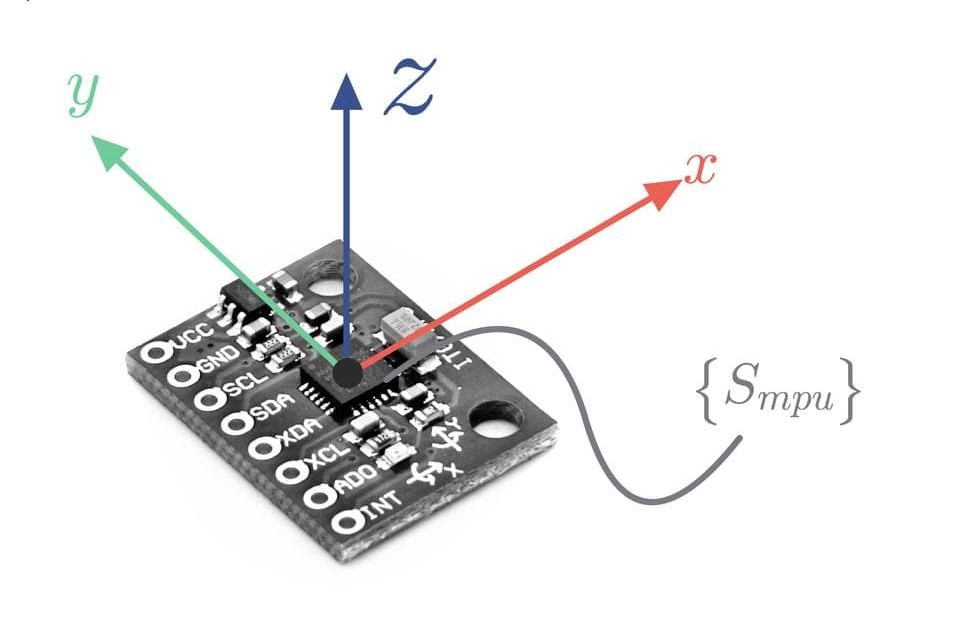
\includegraphics[scale=0.35]{immagini/IMU_sdr.jpg}
    \centering
    \caption{Sistemi di riferimento \textit{body} su una IMU.}
\end{figure}

\clearpage